%This work is licensed under the Creative Commons License Attribution 4.0 International (CC-BY 4.0) 
%https://creativecommons.org/licenses/by/4.0/legalcode 
\documentclass[rgb]{standalone}
\usepackage{tkz-euclide}
\begin{document}
	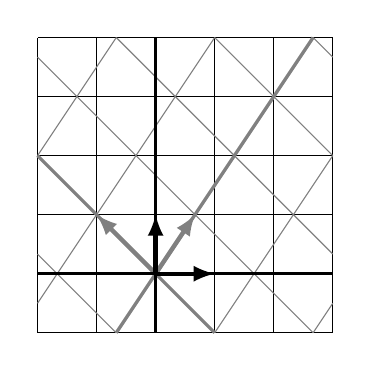
\begin{tikzpicture}[scale=0.5, font=\Large]
		\draw[draw=none] (-3.25,-1.75) -- (-3.25,6.25) -- (4.75,6.25) -- (4.75,-1.75) -- cycle;
		\foreach \i in {-2,...,3}
		{
		\draw[thin] (1.5*\i,-1.5) -- (1.5*\i,6);
		\draw[thin] (-3,1.5*\i+1.5) -- (4.5,1.5*\i+1.5);
		}
		\draw[thin, gray] (-1,-1.5) -- (-3,0.5);
		\draw[thin, gray] (4,-1.5) -- (-3,5.5);
		\draw[thin, gray] (4.5,0.5) -- (-1,6);
		\draw[thin, gray] (4.5,3) -- (1.5,6);
		\draw[thin, gray] (4,6) -- (4.5,5.5);
		\draw[thin, gray] (-3,-0.75) -- (1.5,6);
		\draw[thin, gray] (-3,3) -- (-1,6);
		\draw[thin, gray] (1.5,-1.5) -- (4.5,3);
		\draw[thin, gray] (4,-1.5) -- (4.5,-0.75);
		\draw[very thick, gray] (1.5,-1.5) -- (-3,3);
		\draw[very thick, gray] (-1,-1.5) -- (4,6);	
		\draw[ultra thick, gray, -latex] (0,0) -- (-1.5,1.5);
		\draw[ultra thick, gray, -latex] (0,0) -- (1,1.5);
		\draw[ultra thick, -latex] (0,0) -- (0,1.5);
		\draw[ultra thick, -latex] (0,0) -- (1.5,0);
		\draw[very thick] (-3,0) -- (4.5,0);
		\draw[very thick] (0,-1.5) -- (0,6);	
	\end{tikzpicture}
\end{document}